\documentclass{article}

\usepackage[english]{babel}
\usepackage[utf8]{inputenc}
\usepackage{amsmath,amssymb}
\usepackage{parskip}
\usepackage{graphicx}
\usepackage{subcaption}
\graphicspath{{figures/}}

\usepackage[top = 2.5cm, left = 3cm, right = 3cm, bottom = 4.0cm]{geometry}
\usepackage[table]{xcolor}

\newcommand{\tablespace}{\\
[1.25mm]}
\newcommand\Tstrut{\rule{0pt}{2.6ex}} \newcommand\tstrut{\rule{0pt}{2.0ex}} \newcommand\Bstrut{\rule[-0.9ex]{0pt}{0pt}}

\title{Assignment 1 for DGP 486}
\author{Yangyang Li\\
 yangyang.li@northwestern.edu}
\date{\today}

\begin{document}
\maketitle

\section{PCA Plot}

Raw counts refer to the actual number of RNA-seq reads that are mapped to a gene or transcript.
Raw counts are useful when you want to measure the absolute expression levels of genes, as they reflect the amount of mRNA that is present in the sample.
However, raw counts can be influenced by factors such as sequencing depth, sample preparation, etc.

Normalized counts, on the other hand, adjust raw counts to account for technical variation across samples.
Normalized counts are useful when you want to compare the relative expression levels of genes across different conditions, as they remove the effect of technical variation and allow for a fair comparison of gene expression levels.

In summary, if you want to measure absolute expression levels, use raw counts. If you want to compare relative expression levels across samples, use normalized counts.

\begin{figure}[h]
\begin{subfigure}{0.5\textwidth}
	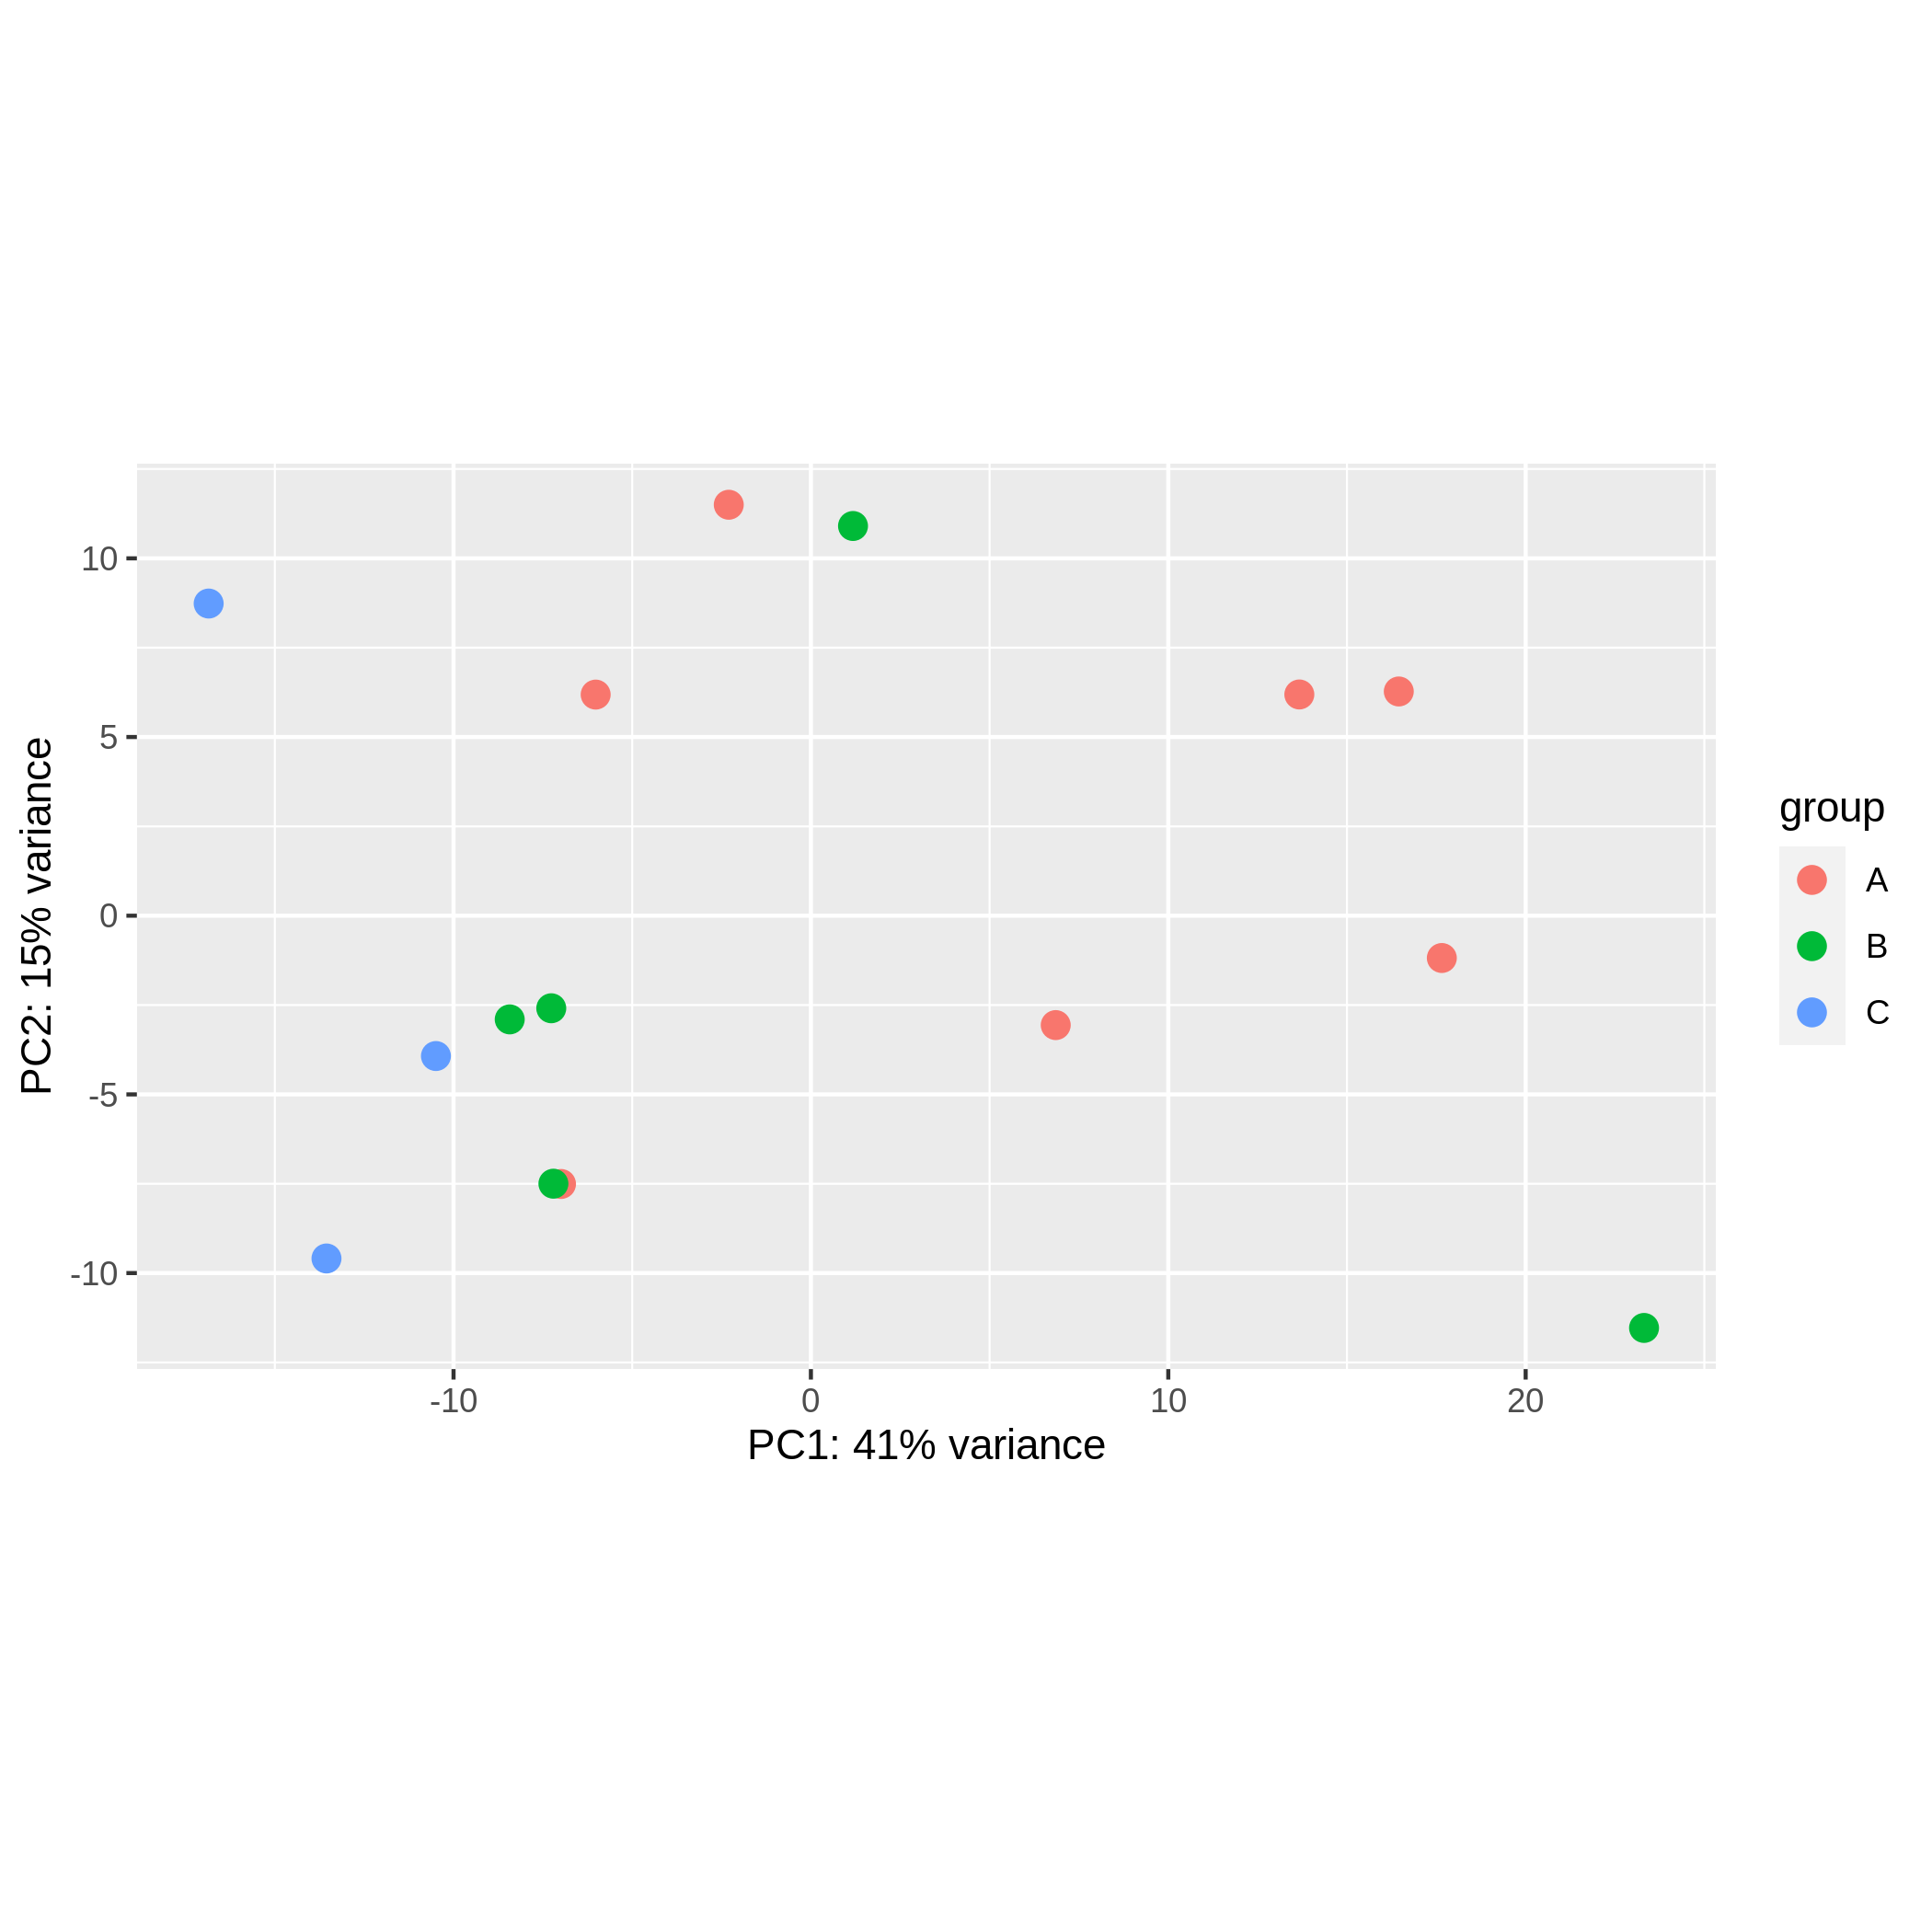
\includegraphics[width = 0.87\linewidth ]{pca_by_batch.png}
	\caption{PCA by Batch}
	\label{fig:pca-by-batch}
\end{subfigure}
\begin{subfigure}{0.5\textwidth}
	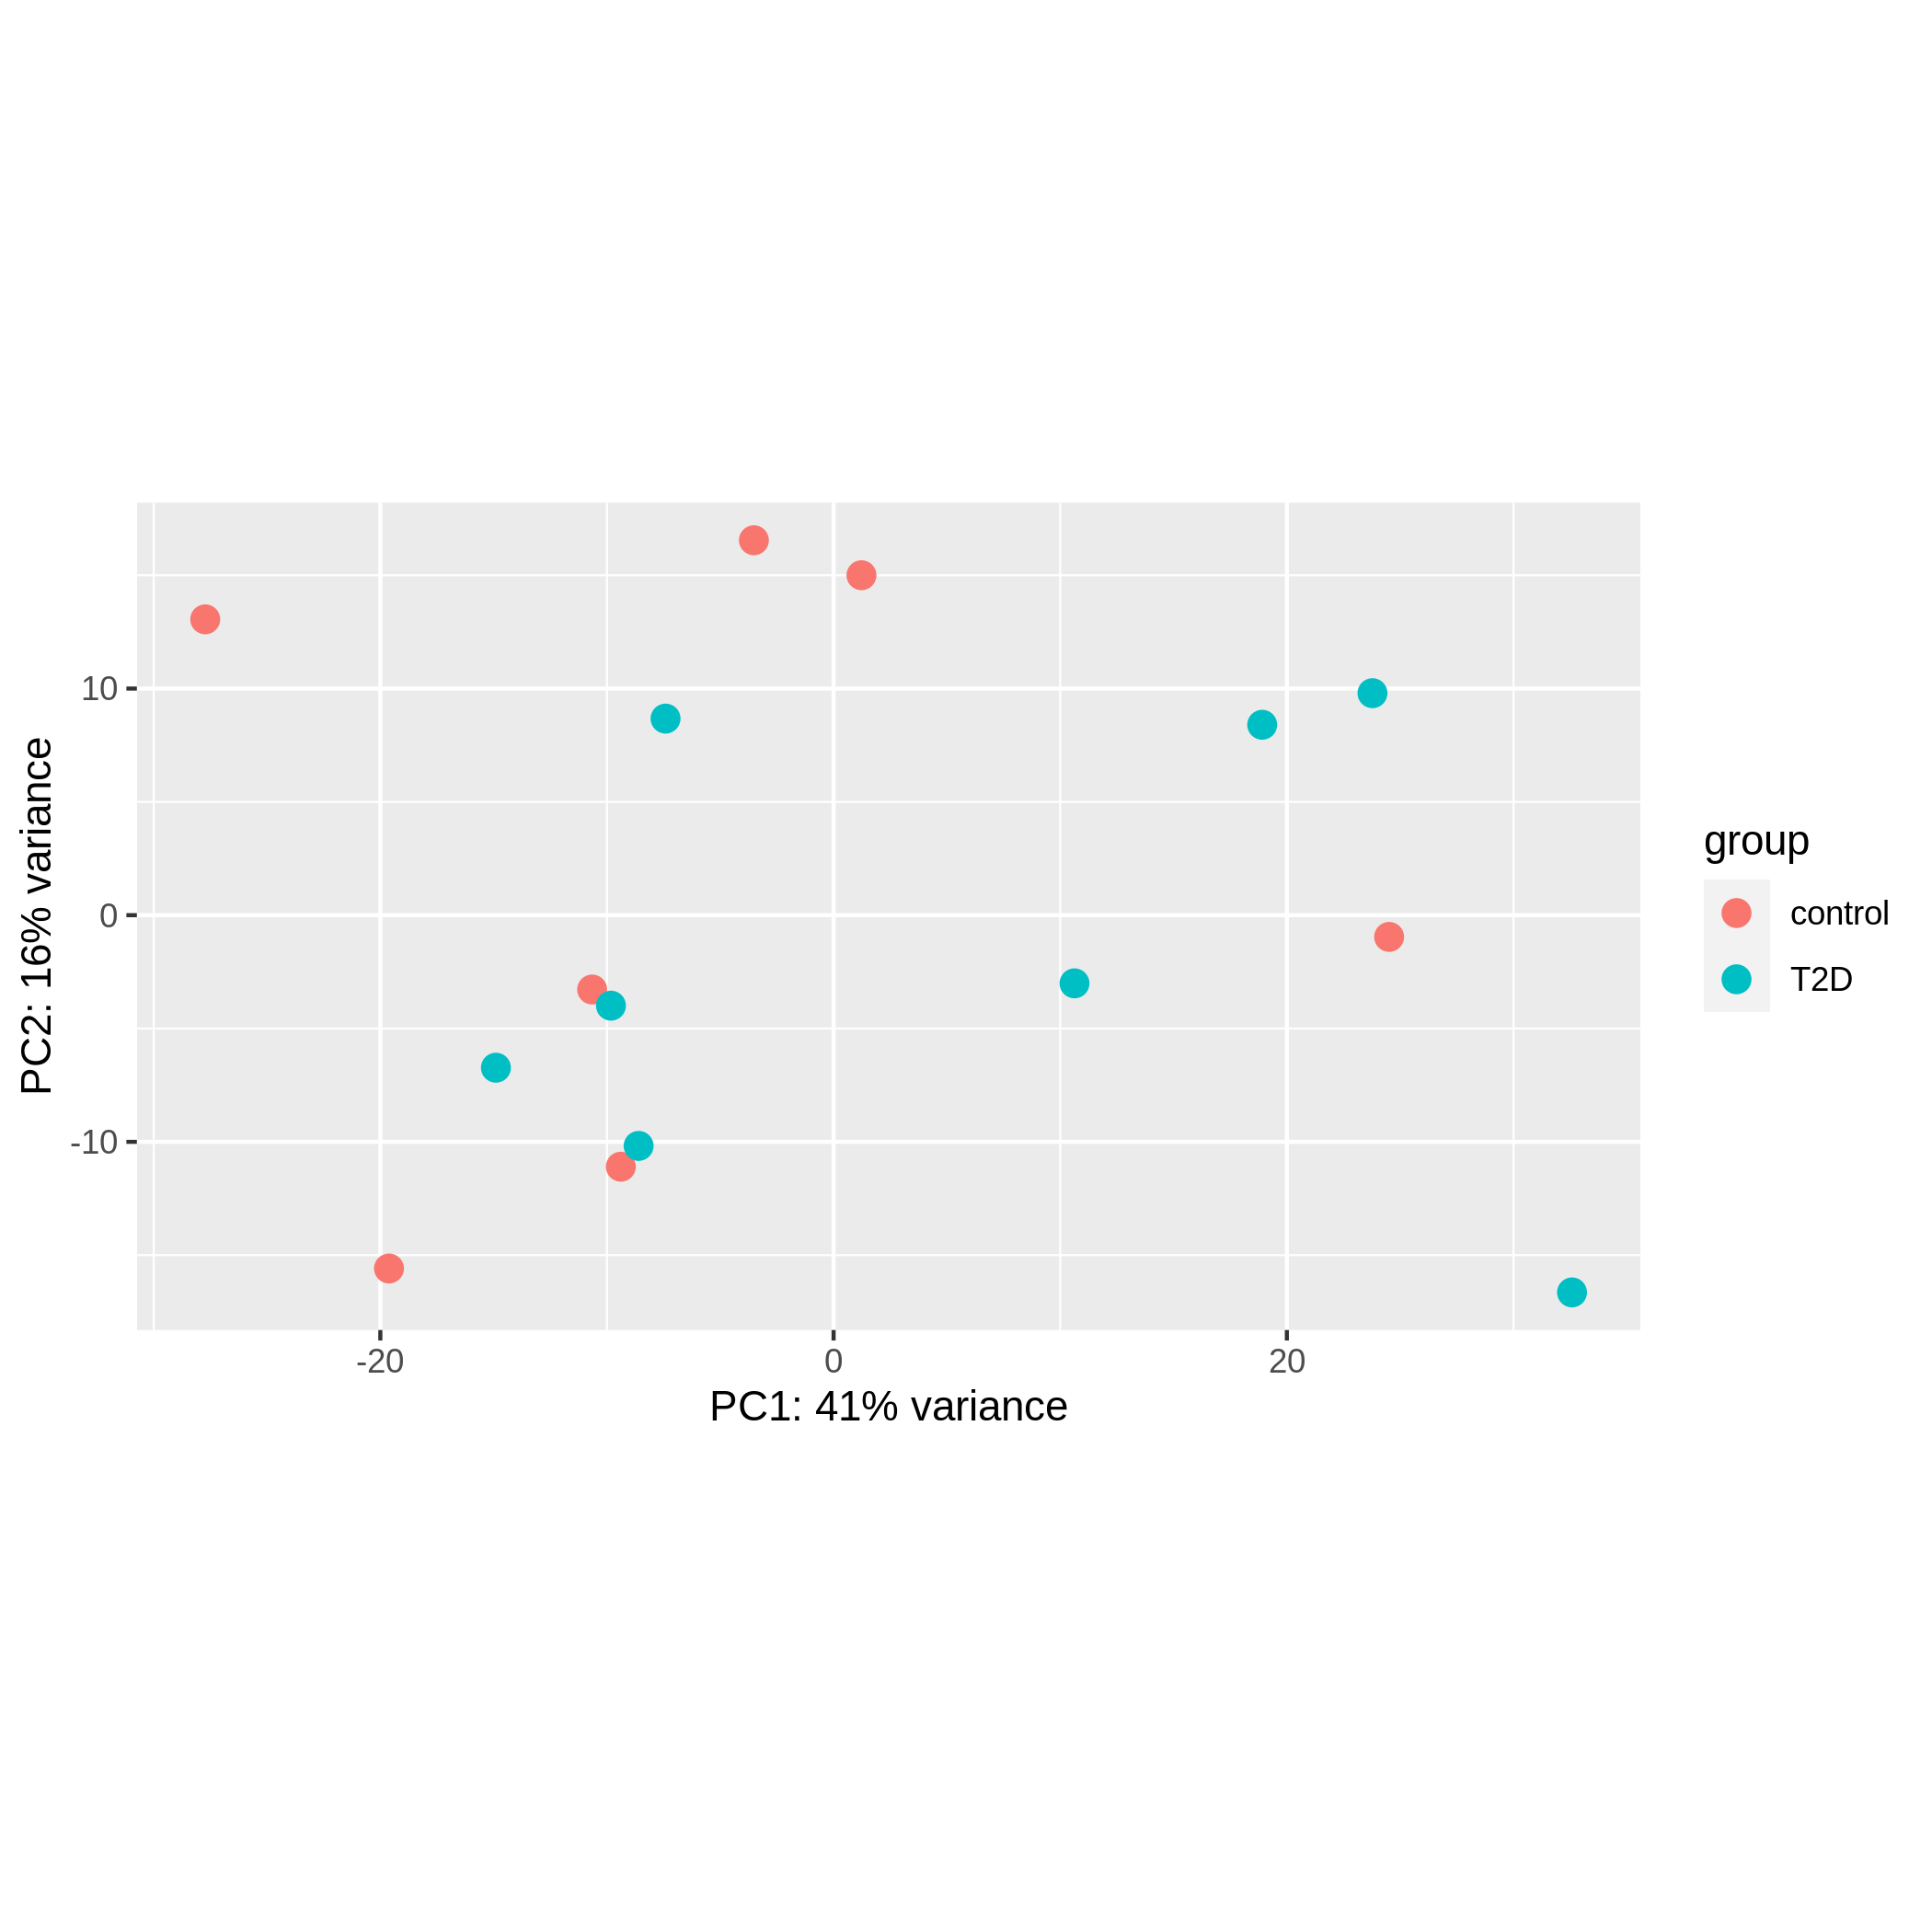
\includegraphics[width = 0.92\linewidth ]{pca_by_group.png}
	\caption{PCA by Group}
	\label{fig:pca-by-group}
\end{subfigure}

\caption{PCA}
\end{figure}


\section{Heatmap}


The Top 10 genes include MIR6723, C1QA, RN7SL3, MIR7641-2, GAMT, SURF1, SLC2A2, TNC, ENTPD3 and TUBB2B.

Among these genes, C1QA (Complement C1q A Chain) is a Protein Coding gene.
Diseases associated with C1QA include C1q Deficiency and Immunodeficiency Due To A Classical Component Pathway Complement Deficiency.
Among its related pathways are Complement cascade and Initial triggering of complement.

GAMT is a Protein Coding gene.
Diseases associated with GAMT include Cerebral Creatine Deficiency Syndrome 2 and Cerebral Creatine Deficiency Syndrome.
Among its related pathways are Gene expression (Transcription) and Creatine metabolism.
Gene Ontology (GO) annotations related to this gene include methyltransferase activity and guanidinoacetate N-methyltransferase activity.


\begin{figure}
	\centering
	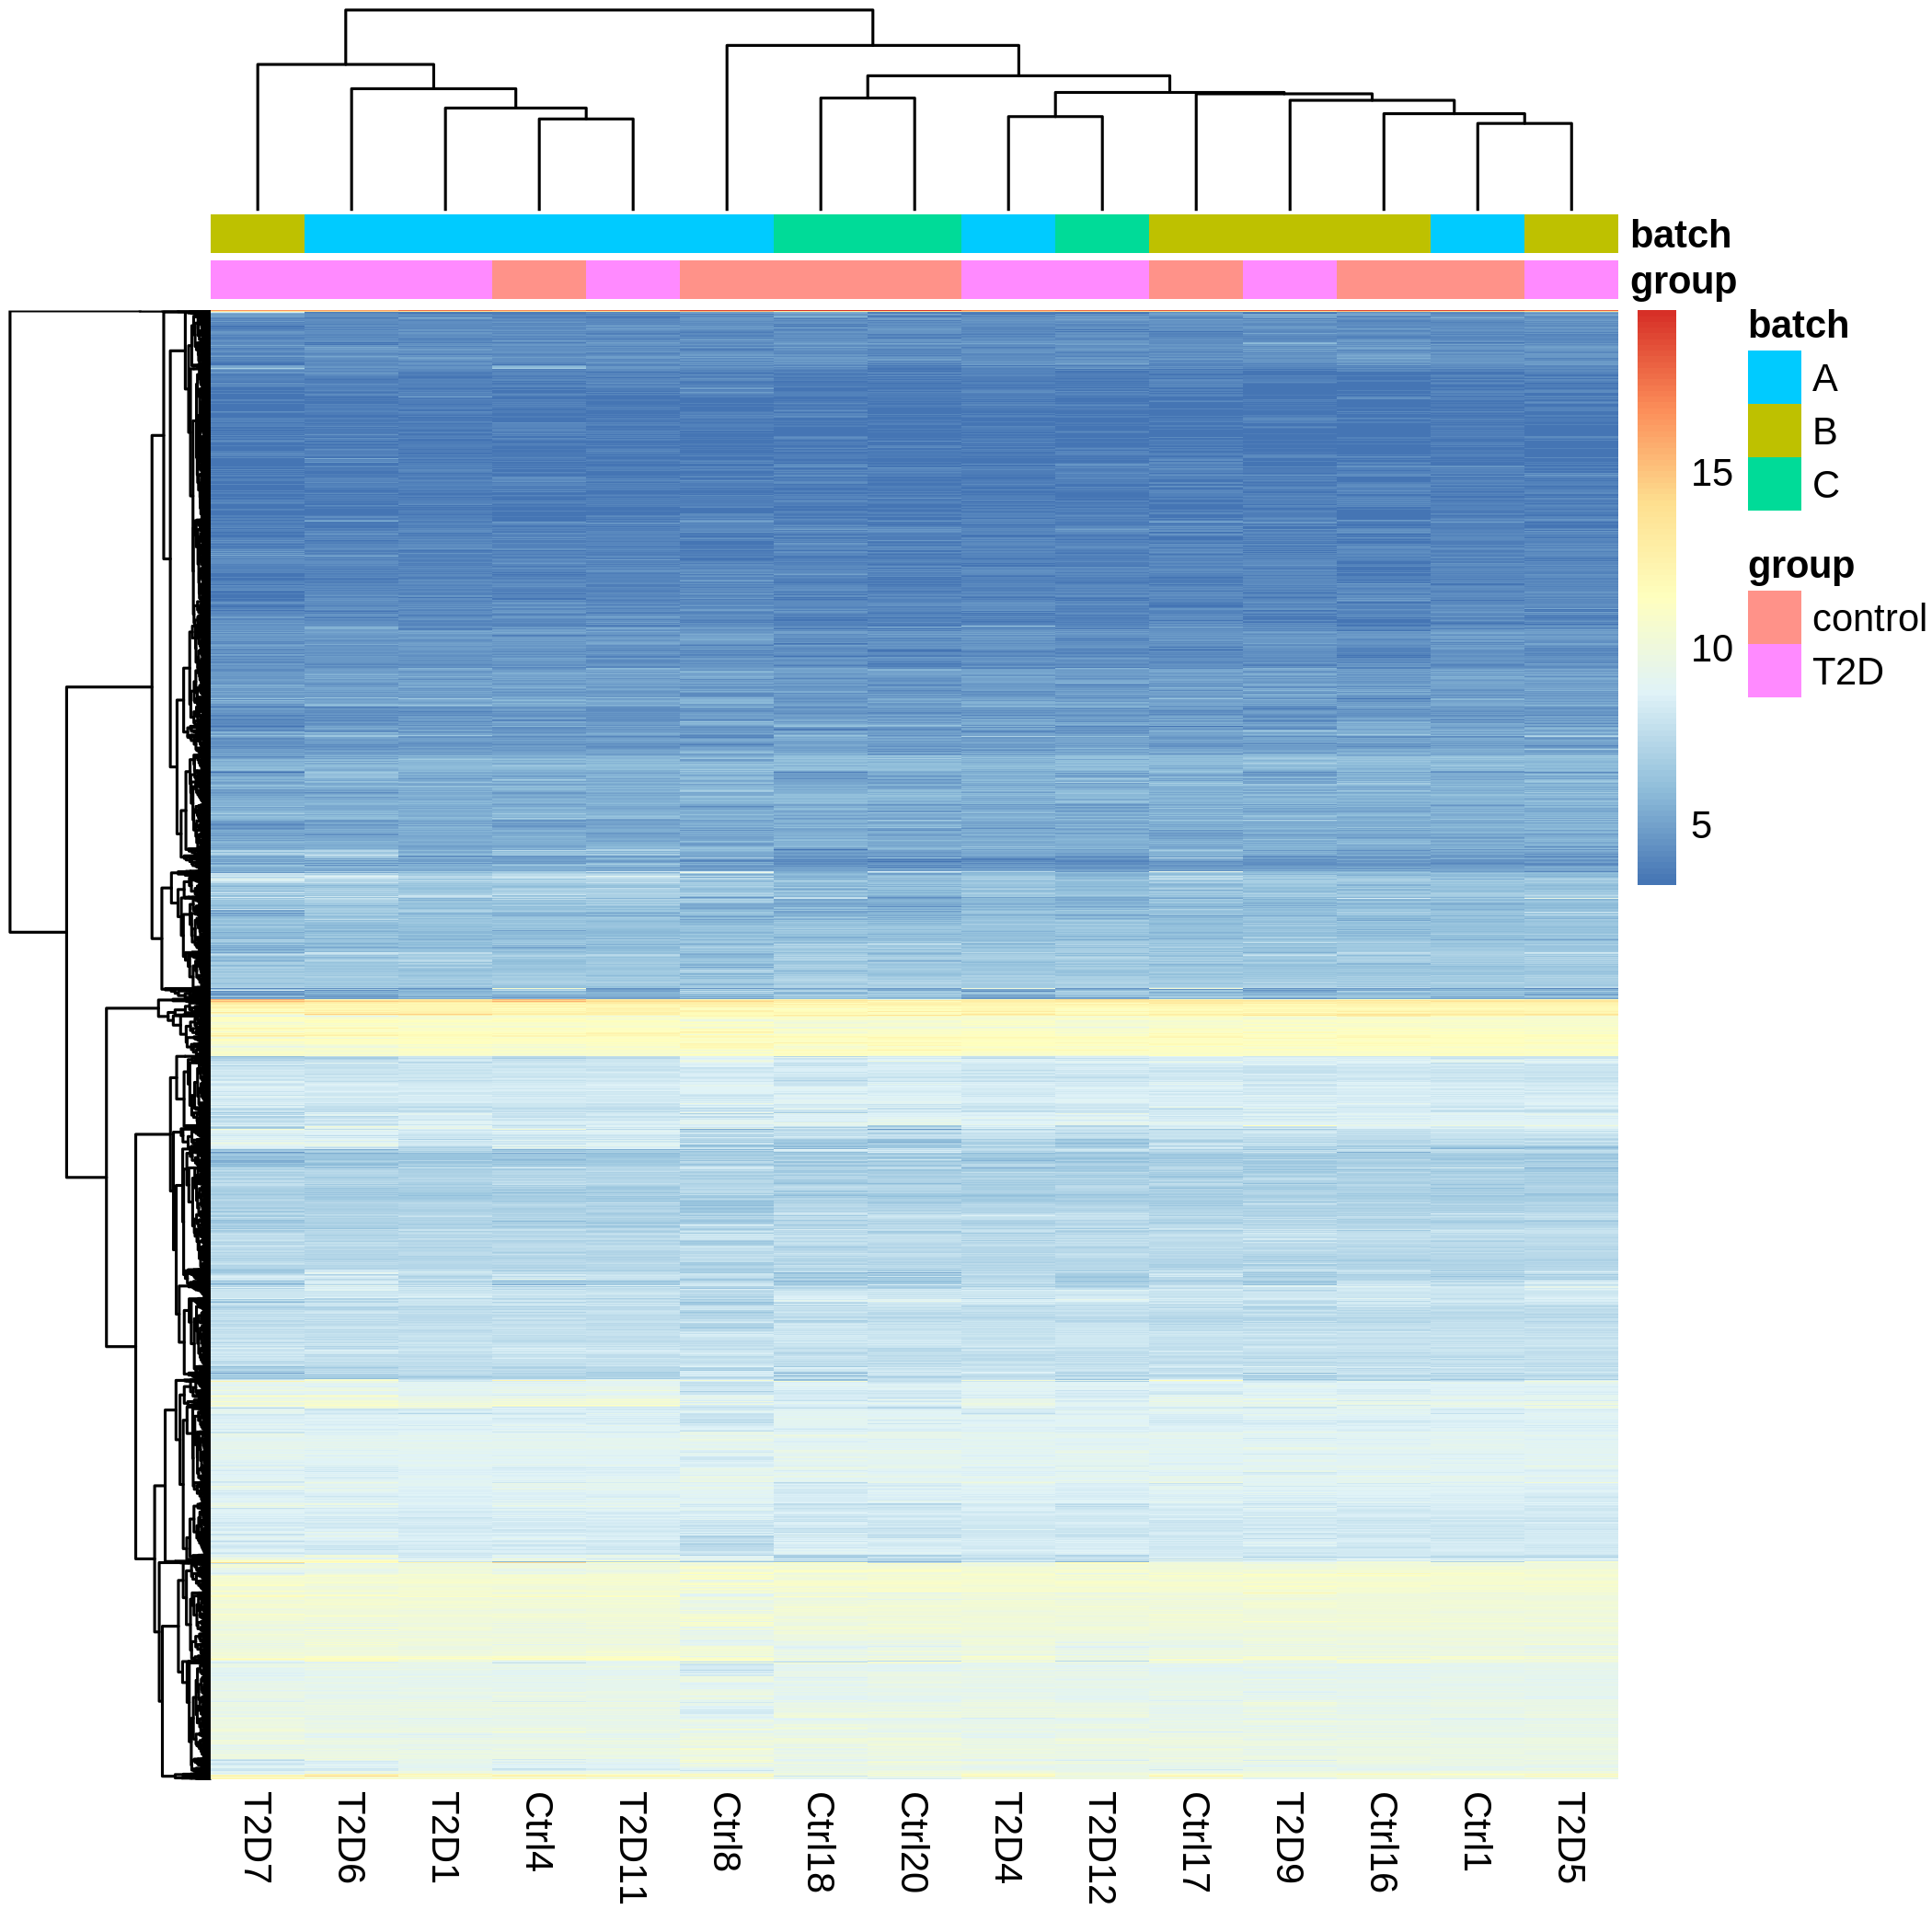
\includegraphics[scale = 0.9]{all_genes_plot.png}
	\caption{Heatmap with all genes}
	\label{fig:heat-all}
\end{figure}


\begin{figure}
	\centering
	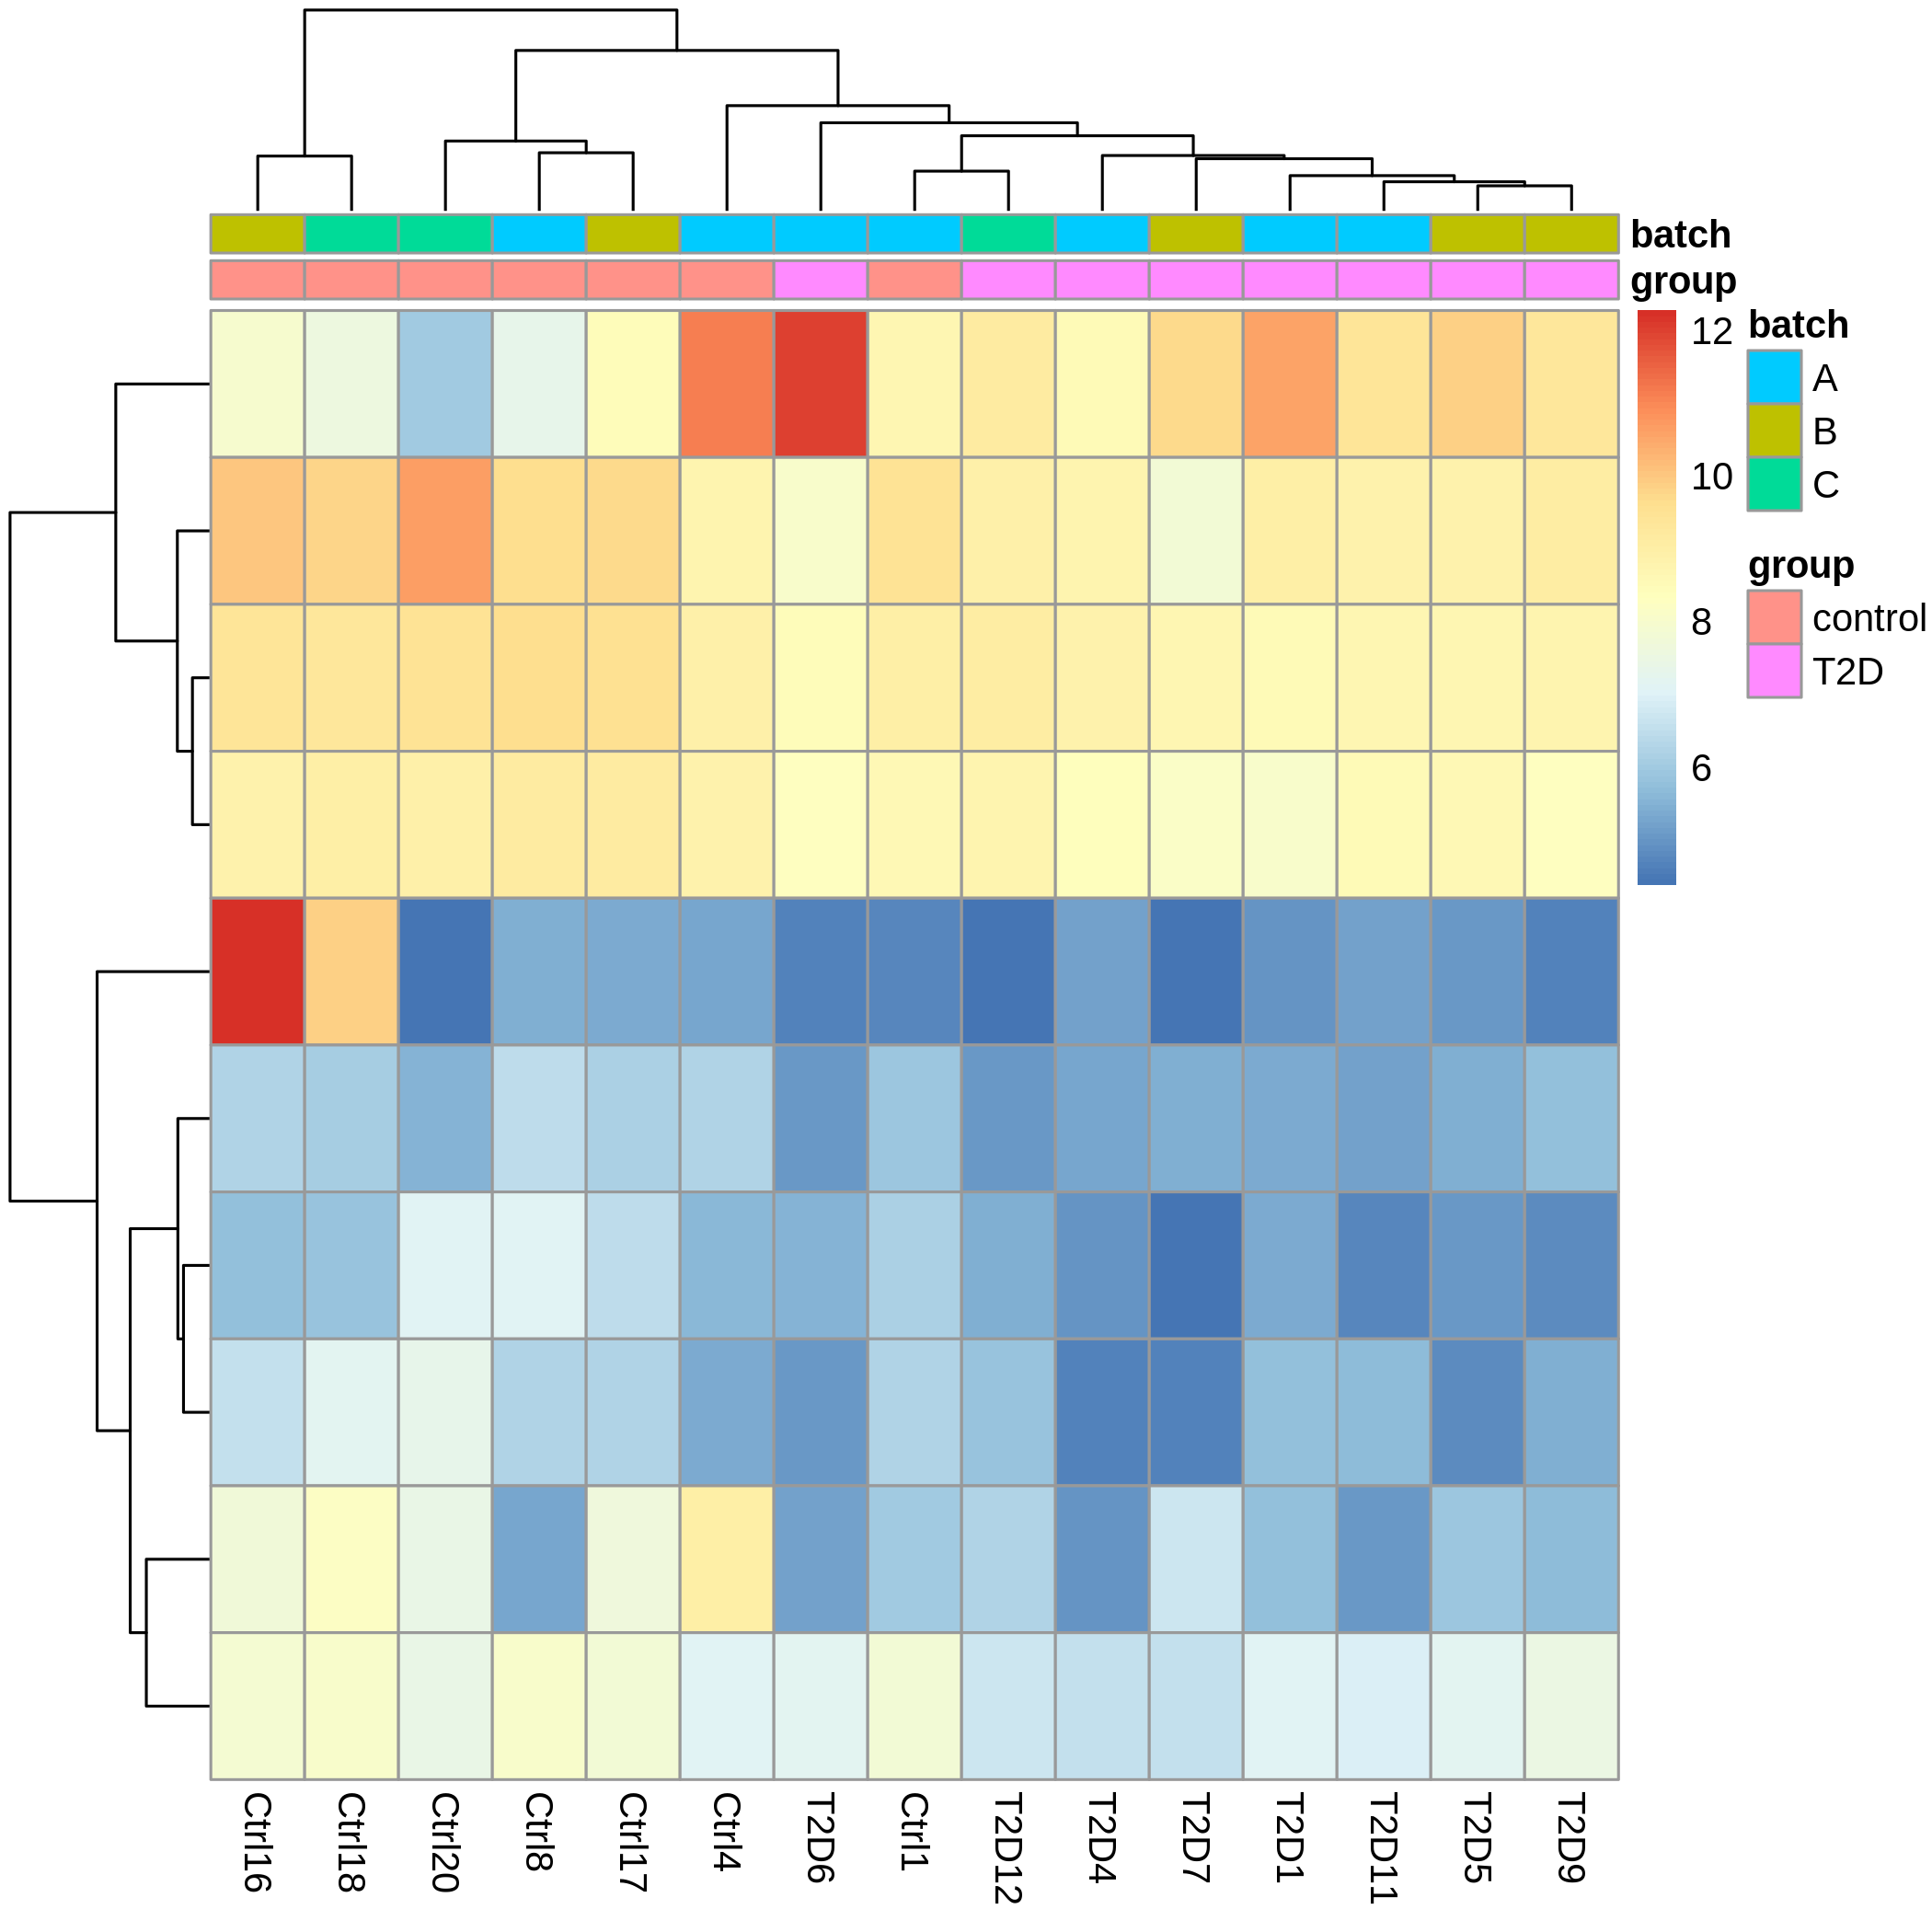
\includegraphics[scale = 0.9]{selected_gene_plot.png}
	\caption{Heatmap with Top 10 genes}
	\label{fig:heat-selected}
\end{figure}


\end{document}
